\section{Neural Geometry Fields (NGFs)}\label{Sec:MainPart}

\subsection{Surface Representation via Quadrangular Patches}

The conventional method for representing 3D surfaces in computer graphics is through triangle meshes, which are collections of vertices connected by triangles that approximate surface geometry. \\
However, this representation presents challenges for machine learning algorithms due to its irregular connectivity and non-uniform structure, making it difficult to process directly with neural networks. \\
Neural Geometry Fields (NGFs) address this issue using a hybrid representation that decomposes surfaces into regular regions suitable for neural network inference while preserving the underlying mesh structure. \\

This hybrid approach begins by dividing the surface of a 3D model into quadrilateral patches, which are four-sided regions that each cover a local area of the geometry. \\
Quadrilaterals are preferred over triangles because they align better with 2D grid parameterizations, enabling each patch to be "unwrapped" and represented as a function over a square domain in 2D space. \\

\usetikzlibrary{calc}
\begin{figure}[ht]
    \centering
    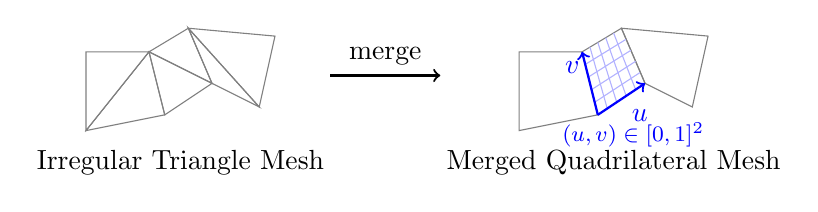
\begin{tikzpicture}
    
        % === Triangle Mesh (Left) ===
        \begin{scope}
          % Nodes
          \coordinate (A) at (0,0);
          \coordinate (B) at (1,0.2);
          \coordinate (C) at (0.8,1);
          \coordinate (D) at (0,1);
          \coordinate (E) at (1.6,0.6);
          \coordinate (F) at (1.3,1.3);
          \coordinate (G) at (2.2,0.3);
          \coordinate (H) at (2.4,1.2);
          
          % Triangle patches
          \draw[gray] (A) -- (B) -- (C) -- cycle;
          \draw[gray] (A) -- (C) -- (D) -- cycle;
          \draw[gray] (B) -- (E) -- (C) -- cycle;
          \draw[gray] (C) -- (E) -- (F) -- cycle;
          \draw[gray] (E) -- (G) -- (F) -- cycle;
          \draw[gray] (F) -- (G) -- (H) -- cycle;
        
          % Label
          \node at (1.2, -0.4) {Irregular Triangle Mesh};
        \end{scope}
        
        % === Arrow ===
        \draw[->, thick] (3.1,0.7) -- (4.5,0.7) node[midway, above] {merge};
        
        % === Quadrilateral Mesh (Right) ===
        \begin{scope}[xshift=5.5cm]
          % Same nodes shifted
          \coordinate (A) at (0,0);
          \coordinate (B) at (1,0.2);
          \coordinate (C) at (0.8,1);
          \coordinate (D) at (0,1);
          \coordinate (E) at (1.6,0.6);
          \coordinate (F) at (1.3,1.3);
          \coordinate (G) at (2.2,0.3);
          \coordinate (H) at (2.4,1.2);
        
          % Merged quadrilateral patches
          \draw[gray] (A) -- (B) -- (C) -- (D) -- cycle;
          \draw[gray] (B) -- (E) -- (F) -- (C) -- cycle;
          \draw[gray] (E) -- (G) -- (H) -- (F) -- cycle;
        
          % Label
          \node at (1.2, -0.4) {Merged Quadrilateral Mesh};

          \begin{scope}
            \clip (B) -- (E) -- (F) -- (C) -- cycle;
            \foreach \u in {0.2,0.4,0.6,0.8} {
                \draw[blue!30] ($(B)!\u!(E)$) -- ($(C)!\u!(F)$);
                \draw[blue!30] ($(B)!\u!(C)$) -- ($(E)!\u!(F)$);
            }
            \end{scope}
          
          % Corrected label axes
        \draw[->, thick, blue] (B) -- ($(B)!1.0!(E)$) node[midway, below right, blue] {\(u\)};
        \draw[->, thick, blue] (B) -- ($(B)!1.0!(C)$) node[midway, above left, blue] {\(v\)};

          
          % Label domain
          \node[blue] at ($(B)!0.5!(F) + (0.3,-0.8)$) {\footnotesize \((u,v) \in [0,1]^2\)};
        \end{scope}
    
        \end{tikzpicture}
        \caption{Conversion of a triangle mesh into quadrilateral patches. The left side shows a simple triangle mesh with marked triangles, and the right shows the surface decomposed into structured quadrilateral patches suitable for parameterization.}
        \label{fig:tri-to-quad}
\end{figure}

Through a process called parameterization (see Figure~\ref{fig:tri-to-quad}), each point on a 3D patch is assigned a pair of 2D coordinates (u,v), where \( u, v \in [0,1] \). \\
This coordinate system allows the surface geometry to be described using continuous functions over regular square domains. \\
As a result, NGFs combine the structured regularity of image-like representations with explicit mesh connectivity, bridging the gap between traditional meshes and fully implicit models such as signed distance fields. \\
By representing a 3D surface as a collection of quadrilateral patches, each with its own local 2D parameterization, NGFs enable precise and expressive surface modeling. \\
This structured format ensures compatibility with neural network architectures, facilitating efficient learning and inference while preserving geometric detail. \\

In practical applications, NGFs do not operate on raw meshes directly. \\
Instead, they rely on preprocessing via quad-remeshing algorithms such as QuadriFlow, which generate an initial decomposition of the surface into quadrilateral patches. \\
These tools provide both a coarse quadrilateral layout and corresponding (u,v) coordinate systems, forming a structured input upon which NGFs can further refine geometry through learning. 
    

%A regular formula

%\begin{equation}
%    x^2 + y^2 = z^2 
%\end{equation}
%and another one
%\begin{equation}
%    \left\Vert \vec{x} \right\Vert = \sqrt{\sum_{i=0}^{n}{x_i^2 + y_i^2}}.
%\end{equation}

%Here is something with matrices:
%\begin{equation}
%\bf{A}=
%\begin{bmatrix}
%    a & b & c\\
%    d & e & f\\
%\end{bmatrix}^\top.
%\end{equation}

%An some inline stuff $\sum a_i=\bf{B}$.

%\begin{table}
%    \caption[List of Symbols]{Keep a list of symbols in your paper.}
%    \label{tab:ListOfSymbols}
%    \resizebox{\columnwidth}{!}
%    {
%    \input{tabs/ListOfSymbols.tex}
%    }
%\end{table}